\documentclass{article}
\usepackage{graphicx} % Required for inserting images
\usepackage{hyperref}

\title{Color Blindness}
\author{Aditya Manjunatha }
\date{Btech 22140}

\begin{document}

\maketitle

\section*{Workflow :- }
\begin{enumerate}
    \item Import the required libraries
    \item Data loading and Preprocessing
    Load the reference sequence (chromosome X) and BWT data (last column and mapping).
    Load the 3 million reads from the genome data.
    Replace any 'N' in the reads with 'A' to handle missing nucleotides.
    \item BWT Preprocessing:
    Generate binary and count arrays for characters A, C, G, T from the BWT last column.
    Use these arrays to perform rank and select queries for string matching.
    \item Rank and Select Queries:
    Implement rank and select functions for characters A, C, G, T.
    Use these functions to perform rank and select queries on the binary and count arrays.
    \item String Matching with BWT:
    For each read, split it into three parts first, second, and third.
    Use the BWT backward search via get\_match\_indices to find exact matches for each part of the read.
    Map the matched indices to positions in the reference genome using the map file.
    \item  Alignment of Read Parts:
    Adjust the reference positions for the second and third parts of the read to align them with the first part.
    Identify common matches across all three parts where the entire read matches perfectly.
    Find remaining matches where only parts of the read match potential approximate matches.
    \item Handling Approximate Matches:
    For the remaining matches, check for mismatches by comparing the full read against the reference sequence.
    Allow up to 2 mismatches for approximate matching.
    For each match with up to 2 mismatches, check whether it corresponds to a red or green exon.
    \item Counting Exon Matches:
    Update the count for the red or green exons based on the matches 0.5 for ambiguous, 1 for unambiguous matches.
    \item Determine Color Blindness Configuration:
    After processing all reads, analyze the counts for the red and green exons.
    Determine the most likely red-green gene configuration based on the read mapping results.
    Check if the configuration matches one of the known configurations for color blindness.
    \item Final Decision:
    Based on the final configuration, decide if the individual is color-blind or not.
    
\end{enumerate}
\section{Functions used in code :-}
\subsection{Creating the reads :- }
We take the reads and replace the 'N' with 'A'\\
For every read, we create its reverse complement, which is done by reversing the read and replacing A with T and G with C and vice-versa.
\subsection{construct\_first\_col(bwt\_last\_col)}
Here we construct the first column by sorting the last column and keeping track of the number of A, C, G, T and \$ we see.\\
Returns the first\_col along with the respective counts which will be used later.
\subsection{def compute\_cumulative\_counts(bwt\_last\_col)}
Here we encode the last column with binary arrays so that we can perform the rank and select operations on them. For example wherever we see an A, we replace with a 1, remaining places we keep as 0. We also keep cumulative counts which is designed to keep a running tally of each nucleotide as it appears in the last column of the (BWT). This cumulative tally allows for fast retrieval of the number of occurrences of each nucleotide up to any given position. For every delta indices in the BWT, we append the values of the cumulative counts to the counters of the nucleotides. This sampling provides a memory-efficient way to store cumulative counts while still allowing rapid access to approximate counts across larger spans.
\subsection{Rank Query}
Just as discussed in class, Given a character and an index, we need to find the number of same characters that are above the current character. We exploit the binary arrays and the counter arrays we made in the last function . So if the index is divisible by delta, then we are good. If not we go to the nearest delta checkpoint that is above the current index, then manually count the characters between the checkpoint and the current character.
\subsection{Select\_first\_column}
This is also a simple function becuase of the structure of the first column. We had kept track of the number of A,C,G,T in the beginning. Then given a character and a number, we appropriately find the index of it in the first column.
\subsection{def lies\_under\_gene(index)}
This function just checks and returns whether the starting index of your read lies inbetween which exon in the red or green parts.
\subsection{def get\_read\_band(read) :- Important}
This algorithm was explained very well in class where we essentially read the 'read' from the end and start to find bands in the BWT with the help of 2 rank's and 2 select operations. At the end we will have a band which represents the suffixes in the rederence sequence whose first k characters exactly match the read, where k is the length of the read.\\
\textbf{Example to explain what is happening :-}\\
So suppose the read is ...Gx . So first we take first\_token as x. Then find the band index wrt the 1st column. We then read G and go to last column and find rank of G wrt to band start and end index. We then go to first column and do 2 select queries on G, and the 2 ranks we got. This ouput's me 2 indices in the 1st column which are the indices corresponding to the first and last band index G of last column right ? So this is also a band whose first column elements are all G . In this band is the second column = x?\\
So like this we do over all the tokens in the read and finally we get a band whose first k columns are exactly the read. Where k is length of the read 
\\
This narrows down the possible suffixes in the BWT matrix that match the prefix of the read you're searching for.\\
After processing all characters of the read, you end up with a band in the first column that represents suffixes whose first k characters exactly match the read, where k is the length of the read.\\
This final band gives you the range of indices in the BWT matrix where the read can be found in the reference sequence.\\
so for example if my range of band index is 10-20 this means that my read matches EXACTLY at 11 places in the reference sequence. 
and these 11 places/indices are given in chrX\_map.txt file. So I can now go to these indices and check if the read matches exactly or not.\\
\subsection{def map\_band\_ro\_ref\_seq(band\_start, band\_end)}
So this function, given a band for a read will map the rows of the band to the refernce sequence. \\
This function Gets me all the places(indices) in the reference sequence where the read matches and store them in ref\_seq\_index\_matches.
\subsection{def no\_mismatches(read, start\_pos)}
Given the read and the potential place where it matches in the reference sequence which is given by the map, we check in how many places the read and the refernce sequence differ starting from index.
\subsection{def split\_read(read)}
This function is used to split the read into 3 parts as discussed in class, this is useful for getting approximate matches. If we just used the whole read for matching, then we only get positions where the read matches EXACTLY. But we are soft and allow for 2 mismatches.
\subsection{def matches\_with\_upto\_2\_mismatches() :- Heart of the assignment}
First we initialize our exon scores.\\
We go to every read, split it into 3 segements.The read is split into three segments (to handle approximate matches more flexibly and potentially locate partial matches when the full read doesn't align exactly due to mismatches). Next take each segement and find where he matches in the reference sequence EXACTLY.\\
So we get 3 sets of indices. We merge these 3 arrays of indices.\\
But before merging we smartly do a index correction because if we need to determine if the entire read matches a specific reference position, we need to align all three segments to a single, continuous position within the reference sequence.\\
By subtracting these offsets, each segment’s reference indices are shifted back to where they would begin if the entire read were aligned at that position. This way, when you later consolidate all indices into unique\_positions each index reflects a potential start position of the full read rather than just the individual segments.\\
This correction means we can verify potential alignment of the entire read at fewer, strategically chosen positions (rather than checking every single segment independently).\\
We keep track whether we have found a match or not by using match\_found = False.\\
We then take our whole read and check whether he matches at these indices, allowing for upto 2 mismatches. If the read satisfies the condition at a particular index, then we add the score to the respective exons depending on whether it was an ambiguous or unambiguous match.(0.5 if it matches with both red and green exons , 1 if it matches exclusively) We do the same by going through all the indices in the matching indices array.\\
If we do find atleast one match, then we update match\_found = True and move on to the next index.\\
Suppose we iterate through all the indices and for all of them, the number of mismatches is greater than 2. Then match\_found flag will still be false.\\
This is when we take the reverse complement read of the current read and repeat the same process of splitting into 3 segments and all.\\
If we find atleast one match for the reverse complement read then we update the scores accordingly. If not then we have failed to find a match for the read. And we must move on to the next read.\\
So in the end we would have 2 arrays of scores for the red genes and the green genes.
\section{Determining the configuration :-}
I have not used any probablity method because i honestly dont know what to do. So i have used the method that sir told in class.
\begin{figure}[h]
    \centering
    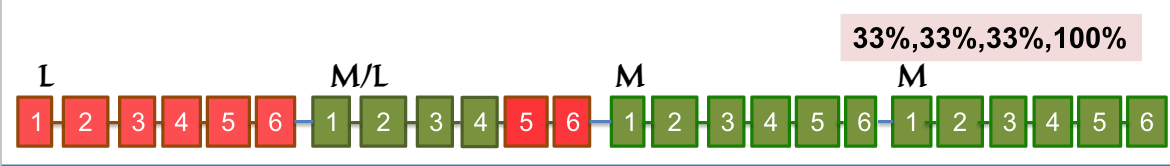
\includegraphics[width=0.8\textwidth]{/Users/adityamanjunatha/Library/CloudStorage/OneDrive-IndianInstituteofScience/IISc Semester/5th Semester/Data Analytics/Assignments/Assignment 5/Report/example.png} % Adjust width as needed
    \caption{Config 4 from slides}
    \label{fig:sample-image}
\end{figure}
Let us look at an example configuration given in class. \\
The 33\% means that the number of reads that matche under Exon 2 of the red gene is 1/3 of the number of reads that match under Exon 2 of the green gene. \\
Similarly for Exon 3, 4, 5. \\
So essentially we have to find out the ratio's of the corresponding exons in the red and green genes. Once we find that out, we need to check to which configurations ratio's is he closest to?
That is exactly what i have done in the code. \\
\section{Partial Results :-}
red\_exon\_scores = [194, 263, 152, 202, 380, 470]\\
green\_exon\_scores = [194, 313, 199, 175, 435, 470]\\
The configuration I got was Configuration 3 :- [0.33, 0.33, 1.0, 1.0]. 
\begin{figure}[h]
    \centering
    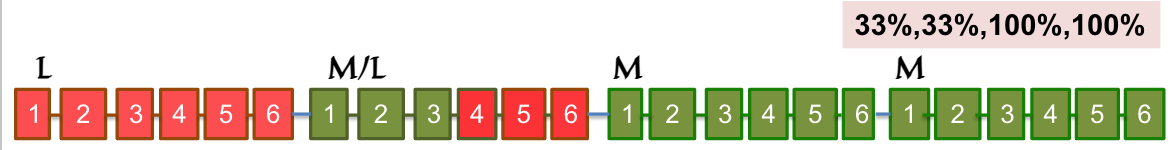
\includegraphics[width=0.8\textwidth]{/Users/adityamanjunatha/Library/CloudStorage/OneDrive-IndianInstituteofScience/IISc Semester/5th Semester/Data Analytics/Assignments/Assignment 5/Report/config.png} % Adjust width as needed
    \caption{Config 3 from slides}
    \label{sample-image}
\end{figure}
\end{document}
